\documentclass[12pt,a4paper]{article}

% --- Pacchetti Standard ---
\usepackage[utf8]{inputenc}
\usepackage[italian]{babel}
\usepackage[T1]{fontenc}
\usepackage{graphicx}
\usepackage{hyperref}
\usepackage{booktabs} % Fondamentale per tabelle di alta qualità
\hypersetup{
    pdfborder={0 0 0} 
}
\usepackage{geometry}
\geometry{margin=2.5cm}

% --- Pacchetto per il Codice ---
\usepackage{listings}
\usepackage{xcolor}

\definecolor{codegray}{rgb}{0.5,0.5,0.5}
\definecolor{codepurple}{rgb}{0.58,0,0.82}
\definecolor{backcolour}{rgb}{0.95,0.95,0.92}

\lstset{
    backgroundcolor=\color{backcolour},
    commentstyle=\color{green!60!black},
    keywordstyle=\color{blue},
    numberstyle=\tiny\color{codegray},
    stringstyle=\color{codepurple},
    basicstyle=\ttfamily\small,
    breaklines=true,
    frame=single
}

\usepackage{fancyhdr}
\pagestyle{fancy}
\setlength{\headheight}{13.6pt}
\fancyhf{}
\fancyhead[L]{\small \textit{MyBarber}} 
\fancyhead[R]{\small \textit{Documentazione }}
\fancyfoot[C]{\thepage} % Numero pagina in basso a destra
\renewcommand{\headrulewidth}{0.4pt} % Linea sotto l'header

\usepackage{titlesec}
\titleformat{\section}
  {\normalfont\Large\bfseries}{\thesection}{1em}{}[{\titlerule[0.5pt]}]

  
% --- Info Documento ---
\title{
    \vspace{-2cm} % Sposta tutto un po' più su per far spazio al logo
    
    
\includegraphics[width=0.25\textwidth]{PDF/logo-unipa.png} \\ % Logo UniPa in alto
    \vspace{0.5cm}
    \textsc{\small Università degli Studi di Palermo}\\
    \textsc{\scriptsize Dipartimento di Ingegneria --- A.A. 2025/2026}\\
    \vspace{1cm}
    \textbf{\huge Documentazione Progetto: MyBarber}
}
\author{Simone Sottile, Giuseppe Giacomarra}
\date{}

\begin{document}


\maketitle


\begin{center}
    \vspace{3cm}
    
\includegraphics[width=0.9\textwidth]{PDF/LOGO.pdf} % Il logo del tuo progetto al centro
\end{center}


\newpage

\tableofcontents
\newpage

\section{Descrizione Generale}
Il progetto \textbf{MyBarber} è una \textbf{Web Application cross-platform} progettata per la digitalizzazione e l'ottimizzazione dei processi di un salone di barberia. Il sistema nasce con l'obiettivo di superare i limiti della gestione manuale degli appuntamenti, offrendo una soluzione centralizzata per due tipologie di utenza:

\begin{itemize}
    \item \textbf{Lato Utente:} Permette ai clienti di prenotare in totale autonomia, selezionando il trattamento desiderato tra le diverse opzioni disponibili — dal taglio classico alla modellatura barba e altri servizi specialistici. Attraverso un calendario dinamico, l'utente può consultare le disponibilità in tempo reale e fissare l'appuntamento istantaneamente, eliminando i tempi d'attesa telefonici e migliorando l'efficienza del salone.
    \item \textbf{Lato Amministratore:} Fornisce al titolare uno strumento gestionale per monitorare l'agenda giornaliera, inserire prenotazioni manuali e avere il pieno controllo sulla disponibilità degli slot. Permette inoltre la gestione dinamica del catalogo, con la possibilità di aggiungere, modificare o rimuovere servizi, prezzi e tempistiche in tempo reale. Include infine funzionalità di reportistica per monitorare l'andamento economico e analizzare i servizi più richiesti, permettendo una pianificazione strategica basata sui dati reali di affluenza e incasso.
\end{itemize}
\subsection{Funzionalità Principali}

\subsubsection{Utente}

\begin{itemize}
    \item \textbf{Gestione Autenticazione:}  Registrazione e login sicuro tramite Token (JWT)
    \item \textbf{Sistema di Prenotazione:} Un modulo interattivo basato su un calendario dinamico. Il sistema interroga il database in tempo reale per filtrare e mostrare esclusivamente gli slot orari ancora disponibili per la data selezionata, prevenendo il fenomeno dell'overbooking.  
    \item \textbf{Gestione appuntamenti:} Una sezione dedicata dove l'utente può monitorare lo stato delle proprie prenotazioni attive e dello storico. Include la funzionalità di cancellazione, che libera automaticamente lo slot orario per altri utenti.
    \item \textbf{Contatti:} Fornisce i dettagli logistici del salone (indirizzo, orari e recapiti). Integra un'interfaccia cartografica basata su \textit{Leaflet.js} per visualizzare la posizione esatta tramite coordinate geografiche.
    \item \textbf{Profilo:} Un'area riservata che permette all'utente di gestire la propria identità digitale all'interno della piattaforma, con la possibilità di aggiornare i dati anagrafici
   \item \textbf{Servizi:} Espone un catalogo digitale interattivo dei trattamenti offerti dal salone. Ogni servizio è presentato tramite una scheda dettagliata che include immagini esplicative, prezzi e tempistiche di esecuzione; il modulo è progettato per guidare l'utente verso la prenotazione consapevole. 
\end{itemize}

\newpage

\subsubsection{Amministratore}

\begin{itemize}
    \item \textbf{Dashboard Gestionale:} Visualizza un riepilogo operativo con incasso giornaliero, servizio più richiesto, prossimo appuntamento e lista dei prossimi appuntamenti confermati.
    \item \textbf{Agenda Appuntamenti:} Permette di consultare le prenotazioni per giorno, settimana o mese, modificare data, ora, servizio e note di una prenotazione già inserita, oppure eliminarla dall'agenda.
    \item \textbf{Prenotazione per Conto Terzi:} Consente di inserire manualmente una prenotazione per un cliente esistente o per un nuovo cliente, selezionando servizio, data, orario disponibile e note. Il sistema controlla gli slot occupati e impedisce sovrapposizioni.
    \item \textbf{Gestione Clientela:} Mostra l'elenco dei clienti registrati con ricerca per nominativo o contatto. Selezionando un cliente, l'amministratore può visualizzarne il dettaglio e lo storico delle prenotazioni.
    \item \textbf{Controllo Disponibilità:} Permette di creare blocchi puntuali su una data o su un intervallo di date, blocchi per intera giornata e regole ricorrenti settimanali. Se il blocco entra in conflitto con appuntamenti già presenti, il sistema richiede conferma e genera notifiche per la riprogrammazione.
    \item \textbf{Analisi Statistiche:} Mostra indicatori sull'andamento del salone, tra cui incassi, appuntamenti, servizi più richiesti e andamento delle prenotazioni nel tempo.
    \item \textbf{Gestione Servizi:} Permette di creare, modificare e disattivare i servizi del listino, configurando nome, descrizione, prezzo, durata, badge, immagine, dettagli e stato di attivazione.
    \item \textbf{Gestione Contatti Salone:} Consente di aggiornare i dati pubblici del salone, inclusi nome, indirizzo, telefono, email, orari, coordinate geografiche e link social.
\end{itemize}

\newpage

\section{Analisi degli Attori}

In questa sezione vengono definiti i soggetti  che interagiscono con la piattaforma \textbf{MyBarber}. Ogni attore ha permessi e modalità di interazione differenti, gestite tramite un sistema di controllo degli accessi basato sui ruoli.

\subsection{Attore: Cliente (User)}
Il \textbf{Cliente} è l'utente finale del sistema. La sua interazione principale avviene tramite l'interfaccia di prenotazione.
\begin{itemize}
    \item \textbf{Obiettivo:} Prenotare un servizio in modo rapido e autonomo.
 
\end{itemize}

\subsection{Attore: Amministratore (Barbiere/Admin)}
L' \textbf{Amministratore} è l'attore che gestisce la logica di business e l'agenda del salone.
\begin{itemize}
    \item \textbf{Obiettivo:} Supervisionare l'agenda e ottimizzare la gestione del tempo di lavoro.

\end{itemize}

\subsection{Database Management System (DBMS)}

Per la persistenza dei dati, il progetto utilizza \textbf{SQLite} come sistema di gestione del database (DBMS).




\newpage

\section{Diagramma Entità-Relazione (ER)}
Il database relazionale SQLite è strutturato secondo il seguente schema aggiornato, coerente con le funzionalità introdotte nel lato amministratore.


\subsection{Modello Entità-Relazione (ER)}
Il modello non si limita più alla sola relazione tra utenti e prenotazioni: l'area amministrativa gestisce anche catalogo servizi, disponibilità, notifiche e dati di contatto del salone.

\begin{itemize}
    \item \textbf{User:} Rappresenta l'anagrafica di chiunque acceda al sistema. All'interno di questa entità, l'attributo \texttt{ruolo} funge da discriminante per l'accesso alle funzionalità amministrative.
    \item \textbf{Prenotazione:} Rappresenta l'appuntamento fissato, contenente data, ora di inizio, ora di fine, durata, stato, note e servizio richiesto.
    \item \textbf{Servizio:} Rappresenta il listino dinamico amministrabile dal barbiere, con prezzo, durata, descrizione, immagine e stato di attivazione.
    \item \textbf{Disponibilità:} Rappresenta i blocchi di agenda inseriti dall'amministratore. Il sistema distingue blocchi puntuali, salvati in \texttt{disponibilita\_blocchi}, e regole ricorrenti, salvate in \texttt{disponibilita\_regole}.
    \item \textbf{Notifica:} Rappresenta i messaggi generati dal sistema per avvisare un cliente quando una prenotazione deve essere riprogrammata.
    \item \textbf{Contatti Salone:} Rappresenta i dati pubblici del salone, modificabili dall'amministratore e mostrati nella sezione contatti.
\end{itemize}

\textbf{Cardinalità principali:} la relazione tra \texttt{users} e \texttt{prenotazioni} è di tipo \textbf{1:N}; un cliente può avere più prenotazioni, mentre ogni prenotazione è associata a un solo utente. Anche \texttt{users} e \texttt{notifiche} sono in relazione \textbf{1:N}. La tabella \texttt{servizi} viene collegata logicamente alle prenotazioni tramite il campo testuale \texttt{valore}: questa scelta consente di mantenere compatibilità con le prenotazioni già salvate, pur permettendo all'amministratore di modificare il catalogo. Le tabelle di disponibilità e contatti salone sono tabelle gestionali usate dall'area admin per controllare gli slot prenotabili e le informazioni pubbliche del salone.

\newpage

\subsection{Modello Logico (Schema SQL)}
In conformità con l'implementazione effettuata tramite il DBMS SQLite, lo schema è così strutturato:


\subsubsection{Tabella: Users}
Contiene i profili utente. Il record relativo al \textit{Barbiere} è pre-configurato con il ruolo amministrativo, mentre le nuove registrazioni vengono impostate di default come clienti.

\begin{table}[h]
\centering

\vspace{1cm}

\begin{tabular}{lll} % Rimosse le linee verticali |l|l|l|
    \toprule
    \textbf{Campo} & \textbf{Tipo} & \textbf{Vincoli} \\ 
    \midrule
    id             & INTEGER       & Primary Key, Autoincrement \\ 
    nome           & TEXT          & Not Null \\ 
    cognome        & TEXT          & Not Null \\ 
    email          & TEXT          & Unique, Not Null \\ 
    password       & TEXT          & Not Null (Criptata) \\ 
    telefono       & TEXT          & --- \\ 
    ruolo          & TEXT          & Default 'user' (admin per il barbiere) \\ 
    \bottomrule
\end{tabular}
\caption{Specifiche tecniche tabella Users}
\end{table}


\subsubsection{Tabella: Servizi}
Contiene il catalogo dei trattamenti mostrati all'utente e modificabili dall'amministratore.

\begin{table}[h!]
\centering
\vspace{0.4cm}
\begin{tabular}{lll}
    \toprule
    \textbf{Campo} & \textbf{Tipo} & \textbf{Vincoli} \\
    \midrule
    id             & INTEGER       & Primary Key, Autoincrement \\
    valore         & TEXT          & Unique, Not Null \\
    nome           & TEXT          & Not Null \\
    descrizione    & TEXT          & --- \\
    prezzo         & REAL          & Not Null, Default 0 \\
    durata\_minuti & INTEGER       & Not Null, Default 30 \\
    badge          & TEXT          & --- \\
    immagine       & TEXT          & --- \\
    dettagli       & TEXT          & --- \\
    attivo         & INTEGER       & Not Null, Default 1 \\
    \bottomrule
\end{tabular}
\caption{Specifiche tecniche tabella Servizi}
\end{table}

\newpage

\subsubsection{Tabella: Prenotazioni}
Memorizza le prenotazioni effettive e mantiene il vincolo di integrità con la tabella utenti.

\begin{table}[h!]
\centering

\vspace{0.4cm}

\begin{tabular}{lll}
    \toprule
    \textbf{Campo} & \textbf{Tipo} & \textbf{Vincoli} \\ 
    \midrule
    id             & INTEGER       & Primary Key, Autoincrement \\ 
    user\_id       & INTEGER       & Foreign Key (\texttt{REFERENCES users.id}) \\ 
    data           & TEXT          & Not Null (Formato YYYY-MM-DD) \\ 
    ora            & TEXT          & Not Null (Formato HH:MM) \\ 
    ora\_fine      & TEXT          & Formato HH:MM \\
    durata\_minuti & INTEGER       & Durata calcolata dal servizio \\
    servizio       & TEXT          & Riferimento logico a \texttt{servizi.valore} \\
    note           & TEXT          & --- \\ 
    stato          & TEXT          & Default 'confermata' \\
    \bottomrule
\end{tabular}
\caption{Specifiche tecniche tabella Prenotazioni}
\end{table}

\subsubsection{Tabella: Disponibilita\_Blocchi}
Memorizza blocchi puntuali dell'agenda, usati per impedire nuove prenotazioni su una data o su una fascia oraria specifica.

\begin{table}[h!]
\centering
\vspace{0.4cm}
\begin{tabular}{lll}
    \toprule
    \textbf{Campo} & \textbf{Tipo} & \textbf{Vincoli} \\
    \midrule
    id                  & INTEGER & Primary Key, Autoincrement \\
    data                & TEXT    & Not Null \\
    ora\_inizio         & TEXT    & Not Null \\
    ora\_fine           & TEXT    & Not Null \\
    intera\_giornata    & INTEGER & Not Null, Default 0 \\
    motivo              & TEXT    & --- \\
    created\_at         & TEXT    & Default CURRENT\_TIMESTAMP \\
    \bottomrule
\end{tabular}
\caption{Specifiche tecniche tabella Disponibilita\_Blocchi}
\end{table}

\newpage

\subsubsection{Tabella: Disponibilita\_Regole}
Memorizza regole ricorrenti di indisponibilità, ad esempio chiusure settimanali o periodi non prenotabili.

\begin{table}[h!]
\centering
\vspace{0.4cm}
\begin{tabular}{lll}
    \toprule
    \textbf{Campo} & \textbf{Tipo} & \textbf{Vincoli} \\
    \midrule
    id                  & INTEGER & Primary Key, Autoincrement \\
    giorno\_settimana   & INTEGER & Not Null \\
    ora\_inizio         & TEXT    & Not Null \\
    ora\_fine           & TEXT    & Not Null \\
    intera\_giornata    & INTEGER & Not Null, Default 0 \\
    motivo              & TEXT    & --- \\
    valida\_dal         & TEXT    & --- \\
    valida\_al          & TEXT    & --- \\
    attiva              & INTEGER & Not Null, Default 1 \\
    created\_at         & TEXT    & Default CURRENT\_TIMESTAMP \\
    \bottomrule
\end{tabular}
\caption{Specifiche tecniche tabella Disponibilita\_Regole}
\end{table}


\subsubsection{Tabella: Notifiche}
Memorizza gli avvisi destinati ai clienti, in particolare quando un blocco di disponibilità rende necessario riprogrammare un appuntamento.

\begin{table}[h!]
\centering
\vspace{0.4cm}
\begin{tabular}{lll}
    \toprule
    \textbf{Campo} & \textbf{Tipo} & \textbf{Vincoli} \\
    \midrule
    id                & INTEGER & Primary Key, Autoincrement \\
    user\_id          & INTEGER & Foreign Key (\texttt{REFERENCES users.id}) \\
    prenotazione\_id  & INTEGER & Foreign Key (\texttt{REFERENCES prenotazioni.id}) \\
    titolo            & TEXT    & Not Null \\
    messaggio         & TEXT    & Not Null \\
    letta             & INTEGER & Not Null, Default 0 \\
    created\_at       & TEXT    & Default CURRENT\_TIMESTAMP \\
    \bottomrule
\end{tabular}
\caption{Specifiche tecniche tabella Notifiche}
\end{table}

\newpage

\subsubsection{Tabella: Contatti\_Salone}
Contiene un solo record con le informazioni pubbliche del salone visualizzate nella pagina contatti.

\begin{table}[h!]
\centering
\vspace{0.4cm}
\begin{tabular}{lll}
    \toprule
    \textbf{Campo} & \textbf{Tipo} & \textbf{Vincoli} \\
    \midrule
    id             & INTEGER & Primary Key, CHECK (id = 1) \\
    nome           & TEXT    & Not Null \\
    indirizzo      & TEXT    & Not Null \\
    telefono       & TEXT    & Not Null \\
    email          & TEXT    & Not Null \\
    orari          & TEXT    & Not Null \\
    latitudine     & REAL    & Not Null \\
    longitudine    & REAL    & Not Null \\
    maps\_url      & TEXT    & --- \\
    instagram\_url & TEXT    & Not Null \\
    facebook\_url  & TEXT    & Not Null \\
    tiktok\_url    & TEXT    & Not Null \\
    updated\_at    & TEXT    & Default CURRENT\_TIMESTAMP \\
    \bottomrule
\end{tabular}
\caption{Specifiche tecniche tabella Contatti\_Salone}
\end{table}

\subsection{Integrità Referenziale e Vincoli}
Il sistema garantisce la coerenza delle informazioni attraverso:
\begin{itemize}
    \item \textbf{Chiave Esterna (Foreign Key):} Il campo \texttt{user\_id} nella tabella prenotazioni assicura che non esistano appuntamenti "orfani", ovvero non associati a un utente reale.
    \item \textbf{Notifiche associate:} Le notifiche mantengono il riferimento all'utente destinatario e, quando necessario, alla prenotazione coinvolta.
    \item \textbf{Unicità dell'Account:} Il vincolo \texttt{UNIQUE} sull'email impedisce registrazioni duplicate.
    \item \textbf{Unicità dello Slot:} L'indice su \texttt{prenotazioni(data, ora)} e i trigger di controllo impediscono la sovrapposizione tra appuntamenti.
    \item \textbf{Disponibilità:} I blocchi puntuali e le regole ricorrenti vengono verificati prima di creare o aggiornare una prenotazione, impedendo la scelta di slot non disponibili.
    \item \textbf{Gestione Date:} Sebbene SQLite non possieda un tipo \texttt{DATE} nativo, l'utilizzo del tipo \texttt{TEXT} con formattazione standard garantisce la possibilità di ordinare cronologicamente i dati lato Backend.
\end{itemize}

\subsection{Rappresentazione Grafica del Modello}
Il seguente diagramma \textit{Entity-Relationship} (ER) riassume la struttura logica aggiornata del database e le relazioni tra le entità coinvolte nella prenotazione e nella gestione amministrativa.

\begin{figure}[h!]
    \centering
    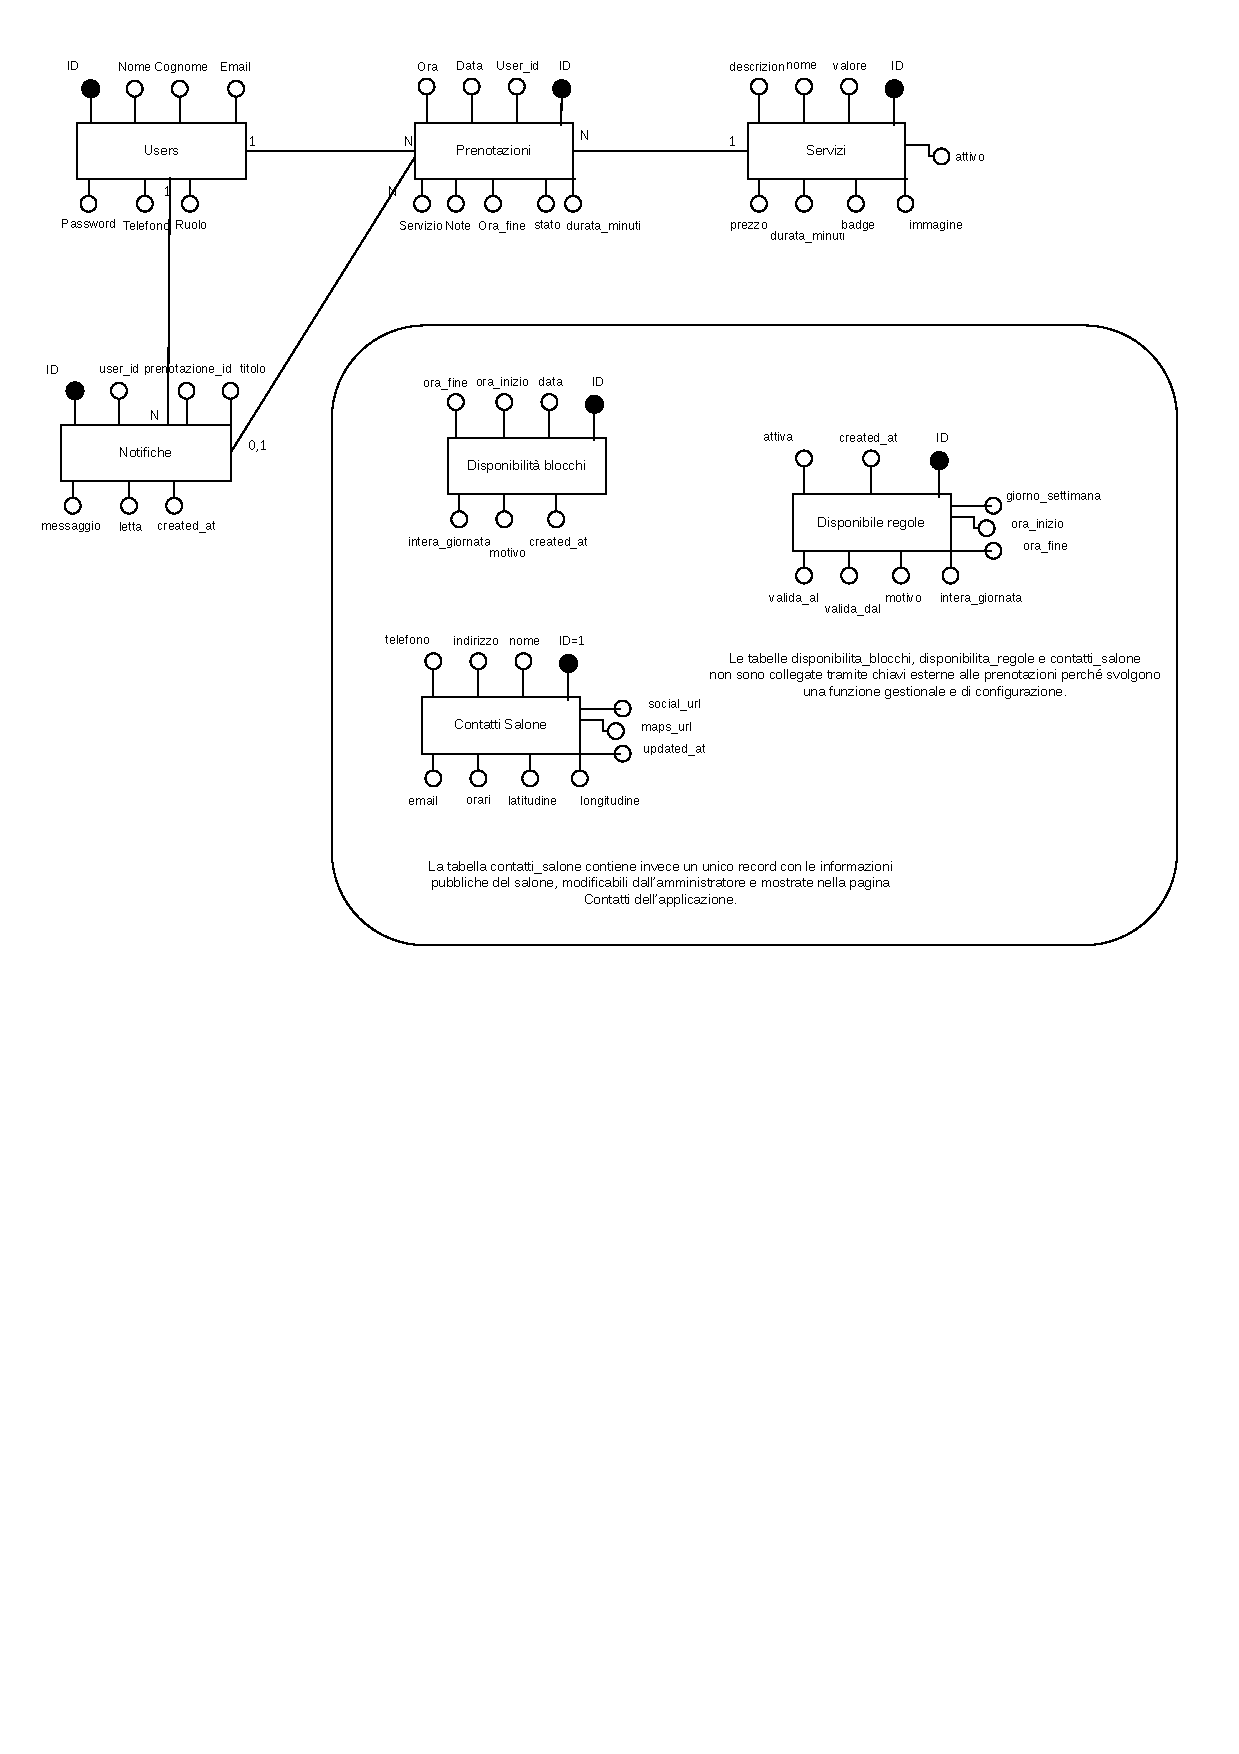
\includegraphics[width=0.85\textwidth]{PDF/ER.pdf} 
    \caption{Diagramma Entità-Relazione.}
    \label{fig:diagramma_er}
\end{figure}
\newpage

\section{Architettura Tecnica}
L'applicazione è basata su uno stack tecnologico moderno:
\begin{itemize}
    \item \textbf{Frontend:} Ionic / Angular.
    \item \textbf{Backend:} Node.js con Express.
    \item \textbf{Database:} SQLite.
\end{itemize}



\end{document}
